\documentclass{ltxdoc}
\usepackage[scheme=plain]{ctex}
\usepackage[style=ieee]{biblatex}
\addbibresource{dev.bib}
\usepackage{array}
\usepackage{tcolorbox}
\tcbuselibrary{skins}

\tcbset{
    enhanced,
    notitle,
    sharp corners,
    colframe=yellow,
    boxrule=1pt,
    center
}

\newtcolorbox{warn}[1][]{
    colback=yellow!5,
    borderline west={2mm}{0mm}{yellow},
    before upper={\textcolor{yellow}{WARNING }},
    #1
}

\usepackage{listings}
\lstset{
    basicstyle=\ttfamily, 
    frame=single, 
    columns=flexible, 
    extendedchars=false
}

\usepackage{multicol}
\usepackage{sjtuvi}
\usepackage{hologo}
\usepackage[colorlinks]{hyperref}

\def\fcmd#1{\paragraph{\fbox{\ttfamily #1}}}

\def\themename{\textsf{SJTUBeamer}}
\def\sjtuglogo{
    
\includegraphics[height=1cm]{sjtug.pdf}
    
\includegraphics[height=1cm]{sjtug_text.pdf}
}

\title{Development Guide of\\\themename}
\author{\sjtuglogo}

\begin{document}
\begin{titlepage}
  \setlength{\parindent}{0em} \addtolength\marginparwidth{-30pt}
  \addtolength\oddsidemargin{-20pt} \addtolength\evensidemargin{-20pt}
  \bfseries\sffamily
  \begin{tikzpicture}[remember picture, overlay]
    \fill[sjtuBluePrimary] (current page.south west)
    rectangle (current page.north east);
  \end{tikzpicture}
  \color{white}\vfill

  \Huge Development Guide of \themename{}

  \Large\LaTeX{} Beamer Template

  \vfill
  \resizebox{!}{2cm}
  {\secondaryinstlogo{
      \resizebox{!}{0.95cm}
      {
\includegraphics{sjtug.pdf}}
    }{\sjtubadge{}}}

  \vfill

  \hskip-9em\resizebox{\paperwidth}{!}{\sjtugate[white]}
\end{titlepage}

\maketitle
\begin{abstract}
  \themename{} is a modular presentation framework based on
  \verb"beamer" class followed by flexible templates dedicated for
  SJTU users. Modern checking systems for \LaTeX\ are adopted over development.
\end{abstract}

\tableofcontents
\clearpage

\section{Contribute}

Welcome to the Development Guide of \themename{}! Before contributing to the
kernel, we highly recommend that you could contribute your first-ever theme
(plugin) to this project before it is solidated to the kernel.

\subsection{Community Version}

You should try out the community version of this beamer template if you want to
maximize the availability. To achieve this, you could download the repo at a
faster speed by making use of the SJTUG mirror source\footnote{You should
  install \href{https://git-scm.com/}{git} first before cloning the repository.}:
\begin{verbatim}
  git clone https://mirror.sjtu.edu.cn/git/SJTUBeamer.git/
\end{verbatim}
After this, to pick up the update from the \verb"main" branch, you could simply
use the command
\begin{verbatim}
  git pull
\end{verbatim}
if you are not using the same main document file aside from
\verb"main.tex"\footnote{Otherwise, there will be conflicts to solve.}.

\subsection{Write a Plugin}

However, you could not make a pull request from a mirror source. The
recommended way is to implement your plugin first. If ready, fork the GitHub
repository \href{https://github.com/sjtug/SJTUBeamer}{sjtug/SJTUBeamer} and
then clone your own fork. Move the modification to your repo and make a pull
request back to the main branch.

\verb"CONTRIBUTING.md" is an outline of how to contribute a plugin to
\themename{}. Refer to it for knowing the basic pipeline on how to contribute.
In a word, enter \verb"src" directory and use
\begin{verbatim}
  l3build add-contrib <plugin>
\end{verbatim}
to initialize a plugin. For more information about this command, see Section
\ref{sec:exclcmd}.

A common template for calling your plugin is as follows:
\begin{verbatim}
  \documentclass{ctexbeamer}
  \usetheme{sjtubeamer}
  \usesjtutheme[<options>]{<plugin>}
  \begin{document}
    % the main content goes here ...
  \end{document}
\end{verbatim}
which will try to insert your \verb"sjtubeamertheme<plugin>.ltx" from the
\verb"contrib/<plugin>" folder, overriding some configurations of the previous
line (\themename\ caller).
\begin{figure}[h]
  \framebox[0.33\textwidth]{\ttfamily main}\framebox[0.33\textwidth]{\ttfamily
    contrib}\framebox[0.33\textwidth]{\ttfamily theme}

  \hfil$\leftarrow$\hfil$\leftarrow$\hfil
\end{figure}

Since the plugin is suffixed by \verb".ltx" (an abbreviation of \LaTeX{}),
which means that it is not recommended to use \verb"@" in the variable. The
plugin is more of a configuration than a basic \LaTeX{} package. If you are
stuck on using such a variable, remember to surround your lines inside the
character-escaped environment:
\begin{verbatim}
  \makeatletter
    \def\foo@bar{bar of foo}
  \makeatother
\end{verbatim}

\themename{} has an internal mechanism of passing the options. For example, if
you pass \verb"debug" option to \verb"sjtug" plugin ---
\verb"\usesjtutheme[debug]{sjtug}",
you could judge the condition in the plugin file like:
\begin{verbatim}
  \if\EqualOption{sjtug}{debug}{true}
    % do something here ...
  \fi
\end{verbatim}
For more information about the customized condition test, see Section
\ref{sec:optdef}. We don't implement the parser for the key-value form, since
it will increase the complexity.

\themename{} has an internal macro on how to include external files in the
contribution path. Use \verb"\getcontribdir{<plugin>}" to get the directory
\verb"contrib/<plugin>" and \verb"\getcontribpath{<plugin>}{<file>}" to get the
directory file path \verb"contrib/<plugin>/<file>". If you are writing the
documentation \verb"<plugin>.tex", the macro could behave differently and sign
a warning. And before writing the documentation, you could refer to Section
\ref{sec:l3build} for how to install the theme on your computer.

\begin{warn}
  We don't recommend using other plugins inside your plugin (native \LaTeX{}
  packages are fine). If you really want to use them, make sure to test your
  documentation to avoid any loop dependency problems.
\end{warn}

However, we could not offer you more about \LaTeX{} or \TeX{} programming aside
from the macros provided by \themename{}. You could refer to the source code of
other plugins for examples. Or you could learn such knowledge from other
references.

\section{Build}

\subsection{Build Overview}

\themename\ has three different types of checking:
\begin{description}
  \item[Regression test] To test the decoupling properties of the modules.
    \texttt{l3build check}
  \item[Unit test] To test each function separately by compiling documentation.
    \texttt{l3build doc}
  \item[CI] To make an overall check by compiling a real-world presentation. It is
    often completed in GitHub Actions when you are pulling a request.
    \texttt{l3build ctan}
\end{description}

\subsection{l3build}\label{sec:l3build}

\themename{} adopts \verb"l3build" system\cite{l3buildman} to build the package. After
entering the source code directory:
\begin{verbatim}
  cd src
\end{verbatim}
You could operate the package by the following command. The build script is set
in \verb"build.lua".

\subsubsection{Built-In Commands}\label{sec:builtincmd}

\fcmd{l3build install} This command will install current version from
\verb"source" to your \TeX{} distribution. Remember to update the
\verb"l3build" to the latest version to avoid misbehaving. This
command requires an argument \verb"--texmfhome" option to specify the
install path, which could be obtained from Mik\TeX{} Console or the
\verb"tlmgr". Then, refresh the database of filenames in your TeX{}
distribution. This command is useful if you want this template to be globally
available for all documents on your computer.

\fcmd{l3build unpack} This command will unpack the source code and create a
sandbox environment in \verb"build/local". You can create your own test
file to test certain features here. It is the most common command for testing a
certain feature.

\fcmd{l3build check} Process a regression test, with an optional parameter to
perform one of the following tests:
\begin{center}
  \ttfamily color font inner outer sjtuvi
\end{center}
which will show if the module is standing-free. If the compilation error
occurs, please check if your code uses one definition from another module
without requiring it first, or an undefined control sequence occurs.

This command will also move the generated style files to the root directory.

\fcmd{l3build doc} This command will generate the documentation of this
package.
% We set an overall testing file \verb"doc/min.tex" to test all features of \themename.
% \begin{center}
%     unpack $\rightarrow$ \verb"min.tex" $\rightarrow$ documentations
% \end{center}
Since the doc has a lot of dependencies (or unit tests), you can cache the demo
files to \verb"support/tutorial" directory. This could be done by the exclusive
\verb"l3build cache-demo" in Section \ref{sec:exclcmd}.
% Change the variable in \verb"build.lua": \verb"cachedemo=true" to cache the demo automatically, and remove the variable to clean the cached files.
% We highly recommend that using *nix to compile the doc.

\fcmd{l3build save color} If you make some modification to the framework
(except \verb"sjtucover") and change the result. To save the current
result as a reference, run this command and \verb"color" could be
exchanged by any of the test units above.

\fcmd{l3build clean} Clean the current \verb"src/build" directory, which
will be useful if you modified one of the temporary files in that directory.
(In this case, you may perform a wrong test with a modified version since
\verb"l3build doc" may not refresh it.)

\fcmd{l3build tag v3.0.0} Tag the version of the source code, which will also
update the date in the source code.

\fcmd{l3build ctan} This is the last step before release. Both
\verb"l3build check" and \verb"l3build doc" will be performed. The
generated file is \verb"src/sjtubeamer-ctan.zip".

More information about \verb"l3build", please refer to
\begin{verbatim}
  texdoc l3build
\end{verbatim}

\subsubsection{Exclusive Commands}\label{sec:exclcmd}

We add a couple of exclusive commands to \verb"l3build" for a better
development experience. These commands are not available in other projects.

\fcmd{l3build cache-demo} This could be used after \texttt{l3build doc}
mentioned in Section \ref{sec:builtincmd} to cache the generated pdf files that
starts with \verb"step". After this command, these pdf's will be
copied to \verb"support/tutorial" directory and will be futher reused in the
next epoch of \verb"l3build doc". To clean the cached demo pdf's, use
\texttt{l3build clean-demo}.

\fcmd{l3build clean-demo} This command will clean the pdf files cached by
\texttt{l3build cache-demo}. It is also recommended to clean all the cached
files before \texttt{l3build add-demo [demonum]}.

\fcmd{l3build add-demo 20} This command will add a new demo file
\texttt{step20.tex} in \texttt{support/tutorial} folder. If the new filename
has been occupied, all the demo files with larger numbers will be renamed (the
number will be incremented in a descending demo number order) to leave the
place for the new file. Notably, the number in the user documentation
\texttt{doc/sjtubeamer.tex} will also be changed. If the corresponding pdf's
are cached, they will get deleted since they are outdated. You need to insert
the description of the new demo in the user documentation later in an
appropriate position.

The file will be generated based on the template
\verb"support/step.template.tex". You could change the demo filename to add
compilation steps in the future \verb"l3build doc" generations. For example,
\verb"step20+.tex" will add another \LaTeX{}\footnote{To decrease the time of
  compilation, the documentation will be compiled in \hologo{pdfLaTeX} on Windows
  and \hologo{XeLaTeX} on Linux and macOS. For more pre-compilation techniques
  that we used in \themename{}, see Section \ref{sec:precompilation}.}
compilation round.

\begin{table}[h]
  \begin{tabular}{cl}
    Symbol   & Description
    \\
    \verb"+" & add another \LaTeX{} round.
    \\
    \multicolumn{2}{c}{\small{\itshape (The following symbols need a premised
    \texttt{+})}}                                             \\
    \verb"-" & add biber compilation before the next \LaTeX{}
    round.                                                    \\
    \verb"_" & add \textsc{Bib}\TeX{} compilation before the
    next \LaTeX{} round.
  \end{tabular}
\end{table}

\fcmd{l3build add-contrib test} This command will create a plugin called
\texttt{test} in the directory \texttt{../contrib}. This command will grab the
information from \texttt{git} to fill the blanks of ``author'' and ``email''
(left blank when no git is installed).

\subsection{Customize Generation}\label{sec:precompile}

In \verb"source/beamerthemesjtubeamer.ins", you could customize what templates
you want to output on the line:
\begin{verbatim}
  \def\preserveoption{,maxplus,max,min,my} 
\end{verbatim}
Reducing the parameter number will reduce the number of templates it generates.
It is useful if you want to debug or make a slight performance jump. Or make
your own version of this template.

\begin{warn}
  \textbf{When you are pulling a request, the item in this column cannot be
    changed}.
  The extraction on your template should be decided by end users since large
  generation files could cause a performance drop on compiling. We are also
  glad to add your template to this column if your template is picked.
\end{warn}

\subsection{Pull Request}

Before making a pull request, please refresh the root \verb".sty" files first
in order to pass CI. In fact, if you are using \verb"l3build", we have embedded
this action in \verb"l3build check" (which is included in \verb"l3build ctan").
But we still recommend that you should make a final run on the script. Switch
to the main directory:
\begin{verbatim}
  cd ..
\end{verbatim}
Then, run the bash code on *nix.
\begin{verbatim}
  .github/ci/build_package.sh
\end{verbatim}

If you are a Windows user\footnote{Windows 10 users could also install WSL
  (Windows Subsystem for Linux) in order to use the Linux environment
  conveniently. This also provides a faster speed on compiling.} and your
\verb"l3build" distribution is not 2021/08/28 and later, please use the old
extracting method in \verb"src/source":
\begin{verbatim}
  latex beamerthemesjtubeamer.ins
\end{verbatim}
and copy the corresponding generated files to the root directory.

\subsection{Continuous Integration}

All other scripts in the folder \verb".github/ci" could also be checked in your
local machine to make sure you can pass the CI on GitHub Actions.

For those who are familiar with \verb"makefile" system, the following commands
might be helpful to build the package under the root directory:

\fcmd{make generate} This command will unpack the Doc\TeX{} files into style
files and update the generated files in the root directory.

\fcmd{make build} This command will build the \verb"main.tex" file.

\fcmd{make build-dev} This command will go through all the tests and generate
the release zip file. You could install the generated \verb".tds"
file into the installing directory of your \TeX{} distribution.

\fcmd{make format-dev} This command will format all the files, and clear the
indent. In order to improve the code quality.

\begin{warn}
  You could download
  \href{https://mirrors.sjtug.sjtu.edu.cn/ctan/support/latexindent.zip}{\ttfamily latexindent} and link the executable path
  \verb"latex-workshop.latexindent.path" in Visual Studio Code.
\end{warn}

\section{Coding Style}

This section gives a contribution code on coding style. Every contributor
should follow this coding style to make a pull request for this project. And
following the coding style strictly will make the Doc\TeX{} compiler for Visual
Studio Code snippets run properly.

\subsection{Framework Code}

The coding style in this section is applicable for the following files:
\begin{verbatim}
  beamerthemesjtubeamer.dtx
  beamercolorthemesjtubeamer.dtx
  beamerfontthemesjtubeamer.dtx
  beamerinnerthemesjtubeamer.dtx
  beamerouterthemesjtubeamer.dtx
  sjtuvi.dtx
\end{verbatim}

\subsubsection{Support Version}

We only support \TeX{} or \LaTeXe{} code on these files. No \LaTeX3 code
supported since \verb"beamer" is not written in \LaTeX3 and this template has a
major dependency on \verb"beamer" class.

\subsubsection{Kernel Function Definition}

The kernel function means that it is not recommended to be used by end users.

\paragraph{If your definition parameters are mandatory, use \TeX\ style.}
This gives you better flexibility on the definition. And in this scenario,
please use a \emph{unique} command name for your function.

\begin{lstlisting}
\def\EqualOption#1#2#3{}
\end{lstlisting}

\subparagraph{Pros:}
Using the bottom layer on \TeX{} gives better processing speed. And making the
parameter declared obviously will make the code more readable, so as the
end-user.

\subparagraph{Cons:}
Using \TeX{} \verb"\def" method will skip the defined macro check provided by
\LaTeX{}, which may cause macro conflict between different packages.

\subparagraph{Decision:}
Use complicated names if you want to avoid naming conflicts on function. This
template won't provide a mandatory rule on this.

\paragraph{If your definition has an optional parameter, use \LaTeX\ style.}
The maximum number of the optional parameter is 1 only. You cannot have more
optional parameters. Give the default optional parameter in the second square
brackets.

\begin{lstlisting}
\expandafter\providecommand\csname #2\endcsname[1][]{}
\end{lstlisting}

\subparagraph{Pros:}
Using this method could get an optional parameter.

\subparagraph{Cons:}
This method is less readable. And have to decide to use \verb"\newcommand"
(check on duplicate functions) or \verb"\providecommand" (no effect if
defined).

\subparagraph{Decision:}
Just use this method if you want an optional parameter. You should not write a
function with more than one optional parameter.

\subsubsection{Interface Function Definition}

Interface function means that the function will be used by end users.

\paragraph{Use \LaTeX\ style on function definition.}
This gives a clear visual indication of the type of this function.

\begin{lstlisting}
\newcommand{\stamparray}[3]{}
    \end{lstlisting}

\subparagraph{Pros:}
This method will avoid the conflict on packages. Or it is easy to debug to know
which package conflicts.

\subparagraph{Cons:}
This method will limit some features \TeX{} provides and you may not pass the
compilation if you switch some \verb"\def" to \verb"\newcommand" or
\verb"\providecommand".

\subparagraph{Decision:}
Use unique name on interface function.

\subsubsection{Global Variable Definition}

Global variable means that it will be used across modules.

\paragraph{Global variables should use the naming scheme as follows.}

\begin{itemize}
  \item Start with the project name \verb"sjtubeamer".
  \item Split by \verb"@" symbol and move to the next level. (only for the middle
        layer)
  \item The final level should be the variable name itself.
\end{itemize}

\begin{lstlisting}
\def\sjtubeamer@inner@lang{en}
\end{lstlisting}

\subparagraph{Pros:}
Make a clear visual indication of the variable type and avoid duplicates with
other packages.

\subparagraph{Cons:}
A long name may make the typing experience troubling and easy to make faults
(hard to check).

\subparagraph{Decision:}
You should avoid using global variables, which will only be useful if you are
making communication between modules. If a bug occurs, it is hard to track in
\LaTeX{}. As a matter of fact, only the parameter in the function can be called
a \emph{local variable} (with an immediate substitution). All variables defined
by \verb"\def" will be stored in the global register.

\subsubsection{Leaf Option Definition}\label{sec:optdef}

Leaf option means it is an option that will not be passed to the next level or
could be used immediately in this module.

\paragraph{Define the package option by an exclusive command, which will define
  a global variable the same as above.}
This will create an option on this package, in package \#1, module \#2, and
variable \#3.

\begin{lstlisting}
\DefineOption{color}{color}{red}
    \end{lstlisting}
which will define \verb"\def\sjtubeamer@color@color{red}" when it receives
\verb"red" option. It is called a leaf option since it will be used in pair
with the following condition test:

\begin{lstlisting}
\if\EqualOption{color}{color}{red}\fi
\end{lstlisting}
which will check if the option is \verb"red".

\subsubsection{Communication Option Definition}

The communication option means it will be a global option passed between
modules.

\paragraph{Declare the variable in an obvious way.}
Use \verb"beamer" macro to declare an option that will not be used in this
module.

\begin{lstlisting}
\DeclareOptionBeamer{red}{\def\sjtubeamer@color{red}}
\end{lstlisting}

\subparagraph{Pros:}
We are making difference between leaf options and communication options in
order to not mess up the communication model. It will make the code much
simpler.

\subparagraph{Cons:}
It is not using \verb"kvoptions" package for a standard option receiver. The
developer has to read the implementation of the macros in \verb"sjtuvi".

\subparagraph{Decision:}
Use our \emph{dialect} of option representation.

\subsection{Cover Code}

The coding style in this section is applicable to the following file:
\begin{verbatim}
  sjtucover.dtx
\end{verbatim}

\subsubsection{Use Beamer Variable}

\paragraph{Use beamer variable to set color and font.}
\verb"beamer" class provides interfaces for using the current configuration
of color and font, see the documentation of \verb"beamer" class
\begin{verbatim}
  texdoc beamer
\end{verbatim}

\begin{lstlisting}
\usebeamercolor{palette primary}
\end{lstlisting}

\subparagraph{Pros:}
Using native macro will provide much more flexibility for your cover template.
It is essential to make your template fit in the color/font management system.

\subparagraph{Cons:}
Developer has to learn how to use these macros and some are not interested in
that.

\subparagraph{Decision:}
To make a pull request, you should always avoid using fixed color/font.

\subsubsection{New Option Declaration}

\paragraph{Copy every region in every file that is marked as \texttt{my} and pastes just below it.} The region is marked as

\begin{verbatim}
  <*my>
  ...
  </my>
\end{verbatim}

Paste it and change \verb"my" to the name of your template. And add the
precompiling option mentioned in Section \ref{sec:precompile}.

\subparagraph{Pros:}
This is useful for template management and end-user could select what template
to be precompiled.

\subparagraph{Cons:}
This is not so handy to search every file. We are working on an automated tool
for developers to achieve that.

\subparagraph{Decision:}
Follow the rule to submit your template.

\subsubsection{Logo Insertion}\label{sec:logoins}

Use a \verb"\resizebox" to resize the logo to the required width and height. If
you want to keep one dimension in the same ratio, use the placeholder \verb"!".

If you want to protect the logo color as the color definition in beamer color
\verb"logo.fg", use \verb"\insertlogo".
\begin{lstlisting}
\resizebox{!}{1cm}{\insertlogo}
\end{lstlisting}

Otherwise, if you want to use the color that is current to the text, use
\verb"\usebeamertemplate{logo}". If you want to modify the current text color,
either use \verb"\usebeamercolor" for beamer color, or \verb"\color" for
regular xcolor.
\begin{lstlisting}
\usebeamercolor[fg]{palette primary}
\resizebox{!}{1cm}{\usebeamertemplate{logo}}
\end{lstlisting}

\subsection{Comment}

Comment means that the ignored lines in the Doc\TeX{} source code.

\subsubsection{Macro Comment}

\paragraph{Start a macro environment to start to comment a macro.}
This environment has one parameter to indicate the name of the macro.

\begin{lstlisting}
% \begin{macro}{\sjtubeamer@color}
    ...
% \end{macro}
\end{lstlisting}

\subsubsection{Macrocode}

\paragraph{To insert source code, you should surround your code with macrocode
  environment.}
This environment must start with four spaces after \verb"%".

\begin{lstlisting}[showspaces=true]
%    \begin{macrocode}
...
%    \end{macrocode}
\end{lstlisting}

\subsubsection{An Example}

Notably, the contents before the \emph{first} \verb"macrocode" environment in
\verb"macro" environment will be treated as the description of this macro. When
generating the Visual Studio Code snippets, the description will be shown. The
searching on the command in \verb"macrocode" environments will decide the
parameter number and the default parameter in the code snippets as well. If you
want to add some notes to this macro, add them before the end of the
\verb"macro" environment. You could use multiple \verb"macrocode" environments
in order to add comments between the code lines.

\begin{lstlisting}[showspaces=true]
%  \begin{macro}{\foobar}
%  <Description of this macro>
%    \begin{macrocode}
<Macro code>
%    \end{macrocode}
%  <Some notes about this macro>
%  \end{macro}
\end{lstlisting}

\section{Framework}\label{sec:framework}

\themename\ is a modular presentation framework. The minimal working files are
listed below. If you want to install \themename{} manually, add these files
into the searching directory of \TeX{} and refresh the filename directory.

\begin{figure}[h]
  \framebox[\textwidth]{\ttfamily main.tex}

  \framebox[\textwidth]{\ttfamily contrib/**/sjtubeamertheme*.ltx}

  \framebox[\textwidth]{\ttfamily beamerthemesjtubeamer.sty}

  \framebox[0.25\textwidth]{\ttfamily
    colortheme.sty}\framebox[0.25\textwidth]{\ttfamily
    innertheme.sty}\framebox[0.25\textwidth]{\ttfamily
    outertheme.sty}\framebox[0.25\textwidth]{\ttfamily fonttheme.sty}

  \parbox[t]{0.25\textwidth}{\centering $\downarrow$}
  \framebox[0.25\textwidth]{\ttfamily sjtucover.sty}
  \parbox[t]{0.25\textwidth}{\centering $\downarrow$} \hspace*{0.25\textwidth}

  \framebox[0.75\textwidth]{\ttfamily sjtuvi.sty}

  \framebox[0.75\textwidth]{\ttfamily vi/*.pdf}
\end{figure}

\subsection{Decoupling}

The framework is designed to be used separately to meet the \verb"beamer" class
requirements on \verb"theme". And any line in the following should be also
available for compilation:
\begin{verbatim}
  \usetheme{sjtubeamer}
  \usecolortheme{sjtubeamer}
  \usefonttheme{sjtubeamer}
  \useinnertheme{sjtubeamer}
  \useoutertheme{sjtubeamer}
  \usepackage{sjtucover}
  \usepackage{sjtuvi}
\end{verbatim}
which requires that the decoupling work between modules should be taken
seriously. The regression test performed by \verb"l3build check" in Section
\ref{sec:l3build} will check such a standard.

\LaTeX{} doesn't load the same style file twice. If the style file is loaded
before, then the next time it loads will get expanded to
\verb"\endinput". Be aware if you are going to load a package twice and
with different options, which will cause an \verb"option clash" error.

\subsection{Communication Model}

The communication model is expanded based on assigning a value to a variable.

\begin{multicols}{2}

  \begin{center}
    \fbox{Declare an option to assign a variable} \par
    $\downarrow$ \par
    \fbox{Set the default configuration} \par
    $\downarrow$ \par
    \fbox{Process the input from the user} \par
    $\downarrow$ \par
    \fbox{Pass the variable to the next module}
  \end{center}

  \begin{flushleft}
    \verb"\DeclareOptionBeamer{max}"\par
    \verb"{\def\sjtubeamer@inner@cover{max}}" \par
    {\centering$\downarrow$ \par}
    \verb"\ExcuteOptionsBeamer{max}" \par {\centering $\downarrow$ \par}
    \verb"\ProcessOptionsBeamer" \par {\centering $\downarrow$ \par}
    \verb"\PassOptionsToPackage"\par\verb"{\sjtubeamer@inner@cover}{sjtucover}"
  \end{flushleft}

\end{multicols}

The table shows the flow of parameter passing.

\begin{table}[h]
  \begin{tabular}{l|>{\ttfamily}l|>{\ttfamily}l>{\ttfamily}l>{\ttfamily}l}
                                    & parent                             &
    color
                                    & inner                              &
    outer                                                                  \\
    \hline
    cover                           & \textbackslash{}sjtubeamer@cover   &
                                    & \textbackslash{}...@inner@cover    &
    \\
    color                           & \textbackslash{}sjtubeamer@color   &
    \textbackslash{}...@color@color & \textbackslash{}...@inner@color    &
    \\
    lum                             & \textbackslash{}sjtubeamer@lum     &
    \textbackslash{}...@clolor@lum  &                                    &
    \\
    lang                            & \textbackslash{}sjtubeamer@lang    &
                                    & \textbackslash{}...@inner@lang     &
    \\
    nav                             & \textbackslash{}sjtubeamer@nav     &
                                    &                                    &
    \textbackslash{}...@outer@nav                                          \\
    logopos                         & \textbackslash{}sjtubeamer@logopos &
                                    &                                    &
    \textbackslash{}...@outer@logopos                                      \\
  \end{tabular}
  \vskip 3pt\moveright 0in\vbox{\hrule width3cm \vskip 3pt
    \moveleft 0em \vbox{
      \hbox{$^{1}$ Since \texttt{font} theme doesn't get any parameters, the
        table omits this column.}
      \hbox{$^{2}$ ... means \texttt{sjtubeamer}.}
    }}
\end{table}

\subsection{Template Management}

About the cover defining method, \themename\ has unified five different covers
into one way of definition --- \verb"\definecover{part}". This macro will
generate two subcommands --- \verb"\partpage" and \verb"\makepart", which is
used to override the original definition with some redundant macros. The
difference between \verb"\make..." series and \verb"\...page" series is that
the former will try to use a \verb"plain" frame in the first place.

\begin{figure}[h]
  \texttt{\textbackslash{}maketitle}\par
  ~~\hspace*{2em}\texttt{\textbackslash{}titlepage}\par
  ~~\hspace*{4em} in sidebar mode, make a left shift\par
  ~~\hspace*{4em} $\hookrightarrow $ insert the defined title page (in
  \verb"sjtucover.sty")\par
\end{figure}

Now, a sandbox in \verb"sjtucover.sty" is created.

To use a different cover style, use
\verb"\setbeamertemplate{title page}[maxplus]" before calling
\verb"\maketitle". The same as \verb"bottom page", \verb"part page",
\verb"section page" and \verb"subsection page". For the sake of simplicity, the
latter three templates could be modified by one parent template
\verb"sectioning pages".

The three types of \verb"sectioning pages" are structured in a way that the
code could be better reused. A typical sectioning page beamer template
definition is as follows.

\begin{verbatim}
  \defbeamertemplate*{sectioning block}{min}[1]{
    % This will define the basic element of sectioning ...
  }
  \defbeamertemplate*{sectioning page}{min}[1]{
    \def\sjtubeamer@cover@sectype{#1}
    \if\EqualOption{cover}{sectype}{subsection}
      \setbeamertemplate{sectioning block}[min]{section}
      \usebeamertemplate{sectioning block}
    \fi
    \setbeamertemplate{sectioning block}[min]{#1}
    \usebeamertemplate{sectioning block}
    \if\EqualOption{cover}{sectype}{part}
      % Some part page specials here ...
    \fi
  }
\end{verbatim}

\themename\ will show the section it belongs to when typesetting the subsection
page, so use \verb"sectioning block" helper template to achieve that. When you
want to override the original \verb"part page" template, use
\verb"\definesecpage{part}{min}" command.

\begin{verbatim}
  \definesecpage{part}{min}
  \definesecpage{section}{min}
  \definesecpage{subsection}{min}
\end{verbatim}

This will redirect to the target \verb"sectioning page" by setting the correct
configuration before using it. This might seems redundant since it has to be
set every time it uses. It seems that the code takes time but actually not,
since it is macro programming for \LaTeX{} and the canonical conditional
changes will only redirect the name of the macro instead of actually pushing
the full data into the register. It is also beneficial for unified management
with the provided macros from \verb"beamer" class.

About the numbering scheme, it uses internal variables to store that, like
\verb"\sjtubeamer@cover@sectionnumber". To adapt to the \verb"ctexbeamer"
class, once it is loaded, the macro will get redirected to the macros defined
in \verb"ctexheading" (remember, if the package \verb"ctex" is loaded
separately, this package will not get loaded). As a result, the user could use
\verb"\ctexset" interface to modify the numbering style after the theme is
loaded (since some modification to \verb"\ctexset" may be introduced in this
theme).

\begin{warn}
  When drawing in the sandbox through Ti\emph{k}Z, make sure to use
  \texttt{overlay} option for adjustment. It will avoid the shift of your cover
  when using \texttt{sidebar} theme.
\end{warn}

Since large source code may cause a performance drop on compiling. We have
figured out a precompiling mechanism to reduce the templates it generates. See
Section \ref{sec:precompile}.

You could also make your customized style by using \texttt{my} option to setup
all components from scratch without leaving the \themename\ ecosystem with all
those utilities.

Developers mainly have two ways to add your template. One is to modify the
source code directly where the placeholder for \texttt{my} style has been left
blank already. The other is to use a new style file \texttt{my.sty} (whatever
the filename) and load it after loading the theme in order to override the
previous settings made by \themename\ itself. And you could use
\texttt{\textbackslash{}setbeamertemplate\{part page\}[maxplus]} to assign the
corresponding template to the existing version. Remember, the placeholder is
all left blank, and if you encountered
\begin{verbatim}
  Divided by zero
\end{verbatim}
errors, you have to assign the placeholder for a correct resizing. And if you
really want to left it blank, use \texttt{\textbackslash{}hphantom\{-\}} or
\texttt{\textbackslash{}vphantom\{-\}} to create a void box.

You could refer to the user guide for a sample file. And the loading on the
package is not that necessary as long as you load the theme before it is
loaded, which is only for the sake of completeness.

\subsection{Logo System}

\themename\ has its own color model on the logo. The main macro is
\verb"\definelogo", which will generate a macro on its file name.

TikZ provides an environment to create our own path fading from picture:
\verb"tikzfadingfrompicture", where you could define your fading in a $(-1,-1)$
to $(1,1)$ rectangle area. Fill the background to black and insert a white logo
in the middle will create a mask. Set the path fading to the name of this mask
will apply to your new TikZ shape.

However, this only creates a square mask. We have to crop it for some
rectangular bounding boxes. Our macro will decide from your input on horizontal
and vertical cropping size for your picture fill the height or fill the width.
And crop the area symmetrically.

\begin{figure}[h]
  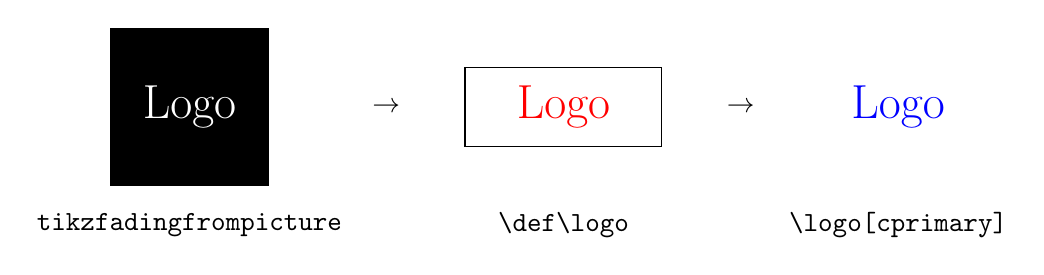
\begin{tikzpicture}
    \draw [fill=black] (-4,1) rectangle (-2,-1);

    \node [white] at (-3,0) {\LARGE Logo};
    \node at (-3,-1.5) {\ttfamily tikzfadingfrompicture};
    \node at (-0.5,0) {$\rightarrow$};

    \draw (0.5,0.5) rectangle (3,-0.5);
    \node [red] at (1.75,0) {\LARGE Logo};
    \node at (1.75,-1.5) {\verb"\def\logo"};
    \node at (4,0) {$\rightarrow$};

    \node [blue] at (6,0) {\LARGE Logo};
    \node at (6,-1.5) {\verb"\logo[cprimary]"};
  \end{tikzpicture}
\end{figure}

Remember, you have to store the picture in a specific folder to create a mask.
It is by default \verb"vi". You could use the optional argument of
\verb"\definelogo" for switching to another folder.

The logo color is now controlled by the current text color. See Section
\ref{sec:logoins} for how to modify the logo color for \verb"\insertlogo".
Otherwise, the generated command can also receive an optional command for
overriding color or changing the opacity or using any supported Ti\emph{k}Z
argument for \verb"\fill". Sometimes, you need to specify the color for your
logo object.

\section{Compatibility}

Since the vision of \LaTeX{} is to build an open-source typesetting system for
multi-platforms and \textsf{beamer} is on top of that to create an
easy-to-configure interface on building presentations, \themename{} follows the
footstep to make its best on compatibility.

\subsection{Beamer Interface}\label{sec:beamer}

\textsf{Beamer} has designed a system of modern interfaces for those theme
creators. \themename{} has already followed the modular architecture, as is
shown in Section \ref{sec:framework}.

And there are more APIs in \textsf{beamer} for each corresponding theme style.
Here is good material about it for a lead-in\cite{tex2017}, which provides a
brief overview. And this part is only focusing on the implementation of
\themename{}. There are mainly three ways to modify a theme:
\begin{enumerate}
  \item \textbf{Want to use presets.} Read Part
        \uppercase\expandafter{\romannumeral3} in the documentation of
        \textsf{beamer}
        package \cite{beamerman}. You can acquire the doc by the terminal
        command:
        \begin{verbatim}
          texdoc beame
        \end{verbatim}
        Then, you could choose to use some preset theme, or call the macro to control
        the appearance of each component.
  \item \textbf{Want a complete modification.} Read the source code of
        \textsf{beamer} package \cite{beamerman}.
        If no additional theme is used,
        \textsf{beamer} will assume you are creating a theme from
        \verb"default". And refer to the corresponding theme file
        suffixed by \verb"default" will give you the bottom
        mechanism to implement components.
  \item \textbf{Want to solve difficult problems.} Go to \TeX{} Stack Exchange
        \cite{texsc} for help. Always search before you ask.
        Then you could probably find some patches and magical
        formulas to tackle the issue since \TeX{} is a
        Turing-complete language.
\end{enumerate}

\subsection{Mainstream Packages}\label{sec:mainstream}

Mainstream \LaTeX{} packages are used to make sure the choice on marcos is
maintained currently. Since some engine doesn't support \textsf{GhostScript}
well (\emph{e.g.} \hologo{XeLaTeX}), \themename{} (as well as \textsf{beamer})
uses \textsc{pgf} as the backend for graphics in \textsf{PostScript}. And half
of the jobs are done on graphics to implement the requirements of VI.

\themename{} doesn't use too many rasterized pictures, since they are not
flexible. You could get the Adobe Illustrator files on VI website\cite{viman}.
SJTU VI goes minimalism so that it could be implemented by package Ti\emph{k}Z
(which is on top of \textsc{pgf}). You could almost draw any vectorized shapes
by referring to Ti\emph{k}Z documentation \cite{tikzman}. In short, Ti\emph{k}Z
uses node-edge system to create graphs and many Computer Science pictures can
be drawn in such a system\cite{tikztuna}. And if you don't want to mess around
with the thousand pages of documentation, Ti\emph{k}ZEdt could help you create
that in a WYSIWYG (what you see is what you get) way\cite{tikzedt}, which is a
tool to make drafts on patterns.

\themename{} also uses additional packages like \textsc{pgfplots} and
\textsc{PgfplotsTable} to draw highly personalized statistic graphs and layout
table from CSV (Comma-Separated Values) respectively. As is mentioned, the
author created a tool \textsc{PgfplotsEdt} to help such graphs in an
interactive way\cite{pgfedt}.

Code blocks are drawn by package \textsf{tcolorbox}, which is also a powerful
toolkit to make customized boxes\cite{tcolorbox}. This is almost the most
elegant way to make colorful boxes in the current \LaTeX{} system.

\subsection{Engine Support}
To be clear, \themename{} is not adapted to all kinds of compilers in the
current \LaTeX{} world.
\begin{table}[h]
  \begin{center}
    \begin{tabular}{ccc}
                           & Windows        & *nix           \\
      pdf\LaTeX{}(C\TeX{}) & $\surd$        &                \\
      pdf\LaTeX{}(CJK)     & $\surd$        & $\surd$        \\
      \hologo{XeLaTeX}     & $\diamondsuit$ & $\surd$        \\
      Lua\LaTeX{}          & $\diamondsuit$ & $\diamondsuit$ \\
    \end{tabular}
    \vskip 3pt\moveright 1in\vbox{\hrule width3cm \vskip 3pt
      \moveleft 0em \hbox{$^*\surd$ is fully available, while $\diamondsuit$
        will have font issues.}
    }
  \end{center}
\end{table}

As always, we strongly recommend compiling the document through
\hologo{XeLaTeX} in Mac and Linux Operating Systems, and pdf\LaTeX{} in
Windows. And Lua\LaTeX{} is pretty slow with \verb"beamer" class, which is not
recommended. But it has \verb"lua-visual-debug" package for developers to check
the bounding box of each component to check errors.

\themename{} make its effort on engine support in the following ways:
\begin{enumerate}
  \item \textbf{Use \textsf{beamer} interface.} As is mentioned in Section
        \ref{sec:beamer}, \themename{} will not create its macro
        unless there is no substitute in the current version of
        \textsf{beamer} or it is a common method to implement some features.
        A good example of this is to make a bottom page,
        \themename{} mimicked \verb"\maketitle" command to implement
        \verb"\makebottom" command. A good outcome is that the style file
        could be separately used with low coupling.
  \item \textbf{Use mainstream packages.} Mentioned in Section
        \ref{sec:mainstream}, mainstream packages are widely accepted in many
        engines.
        Some top-level macros are used to increase the readability of the
        source code,
        i.e., \textsc{pgf} is lengthy and hard to be maintained.
  \item \textbf{Use old-fashioned \TeX{} code.} If there is a nice way to
        implement in \TeX{}, then go \TeX{}. \TeX{} is a box-based typesetting
        system, which may be mentioned in many Computer Science books. And
        \LaTeX{} is on top of that to provide clear-to-read macros. In some
        scenarios,
        the native \verb"\vbox" and \verb"\hbox"
        commands could
        help calculate the position of characters in a more controllable way.
        But it is certainly painful to learn. The \TeX{} Book\cite{texbook} is
        the
        classic to learn that, but Notes On Programming in \TeX{}\cite{texnote}
        is more
        recommended in modern \LaTeX{}.
\end{enumerate}

\subsection{Adaptive Layout}

\themename{} aims at adapting to as many layouts as possible. Since
\themename{} is a decoupled modular part, the layout could be changed due to
external package options. And it should be natively decoupled or adaptive to
the context through adaptive codes instead of code with no hooks.

\begin{enumerate}
  \item \textbf{Options from \texttt{beamer} class to change the size.}
        \themename{} is based on \verb"beamer" class in the bottom
        layer.
        Users could pass options to \verb"beamer" class like
        \verb"12pt" to change the overall font size or
        \verb"aspectratio=169" to change the slide size. This could damage
        the layout of the components like \verb"frametitle",
        covers if its measurement is in unit \verb"cm" or
        \verb"pt" which is not font adaptive.
        We recommend using \verb"em" in width and
        \verb"ex" in height to make it font adaptive.
        Since the default font size of \verb"beamer" is 11pt,
        the following conversion on measurement could
        be inferred \cite{texbook}. Make the conversion when
        transplanting components from other templates (However, the first table
        is only used for 10pt, or \verb"cmr10" font. For the default font size
        11pt, try to use a bigger absolute measurement):

        % TODO: calculate the 11pt sans font result.

        \begin{tabular}{lll}
                     & 1em    & 1ex    \\
          \verb"\rm" & 10pt   & 4.3pt  \\
          \verb"\bf" & 11.5pt & 4.44pt \\
          \verb"\tt" & 10.5pt & 4.3pt  \\
        \end{tabular} \vrule
        \begin{tabular}{>{\ttfamily}ll}
          pt & point                       \\
          pc & pica (1 pc = 12 pt)         \\
          in & inch (1 in = 72.27 pt)      \\
          cm & centimeter (2.54 cm = 1 in)
        \end{tabular}

        However, it is not always meant to use font adaptive \verb"em" and \verb"ex"
        everywhere in your code. You should be aware of some spaces should not be
        adaptive such as the spacing in the drawings. And when it comes to the change
        of aspect ratio, the result should be calculated from the width and height
        geometry instead of hard-coded measurement in most cases.
  \item \textbf{Themes from \texttt{beamer} class.} \themename{} has adapted to
        most of the outer themes provided by \texttt{beamer} class by passing
        the corresponding option. \themename{} aims at providing consistent
        layouts through different outer styles. So, there are some
        modifications
        corresponding to different outer styles after one of them is loaded.
  \item \textbf{Options from \texttt{ctexbeamer} class to change the format.}
        Users could also use \verb"\ctexset{}" provided by
        \verb"ctexbeamer" to change the format of the section number or
        change the font by \verb"fontset=ubuntu". \themename{} has adapted
        to some of the \verb"ctexset" options but the majority of
        them have
        not been adapted since the meaning could get changed from
        \verb"article" class to \verb"beamer" class. Some
        name
        translations are required to
        change from other packages like \verb"algorithm2e". In this
        scenario,
        use \verb"\@ifpackageloaded{}" macro to patch the code manually. And
        sometimes the package will get loaded after the theme, so you are most
        likely to do the patch in \verb"\AtBeginDocument{}".
  \item \textbf{Modifications from contribution plugins.}
        The plugin itself may also change the layout in some ways.
        For example, the \verb"poster" plugin needs to change the
        font measurement and emulate the high DPI behavior.
        The more adaptive the upstream code is,
        the easier modifications of the plugin are.
        Keep it in mind to adapt to as many cases as possible.
\end{enumerate}

\subsection{Old \TeX\ Distribution}

To make full use of \themename\, we always recommend using the latest \TeX\
distribution. However, in some cases, an older \TeX\ distribution needs to be
supported.

For compatibility issues, you need to define the \verb"\sjtubeamer@compatible"
variable to \verb"false" to close the related rendering before the theme is
loaded.

\begin{verbatim}
  \makeatletter
  \def\sjtubeamer@compatible{false}
  \makeatother
\end{verbatim}

\begin{tabular}{c|ccccccccc}
  \TeX\ Live & 2022    & 2021    & 2020    & 2019    & 2018    & 2017    & 2016
             & 2015    & 2014
  \\
  \hline
  Test       & $\surd$ & $\surd$ & $\surd$ & $\surd$ & $\circ$ & $\circ$ &
  $\circ$    & $\circ$ &
  \\
\end{tabular}

\subsection{Pre-Compilation}\label{sec:precompilation}

\themename\ is relatively a large project for developers. To boost up the
compilation on 20+ unit tests, we introduced \texttt{mylatexformat} to cache
the precompiled common header. However, this method comes with compatibility
issues in that it only supports old packages \emph{without} using
\texttt{fontspec} to load OpenType fonts.

To dump the format on \verb"beamer", we have to reset the encoding to the old
7-bit default\cite{mylatexot1}. Since some sans fonts use a newer version. And
it is not available for C\TeX{} in \hologo{XeLaTeX}, since it uses
\texttt{fontspec} to load the font. What's more, if we decided to load
\texttt{ctex} after loading \texttt{ctexbeamer}, the load on \texttt{ctex} will
be skipped\cite{ctex}. And \themename\ has done some work similar to
\texttt{ctexbeamer}. As a result, we need to split the document class loading
line \texttt{\textbackslash documentclass\{ctexbeamer\}} into two parts, which
means the loading time on \texttt{ctex} will not be saved:
\begin{verbatim}
  %--- static -----
  \RequirePackage[OT1]{fontenc}
  \documentclass{beamer}
  %--- dynamic ---
  \endofdump
  \usepackage{ctex}
\end{verbatim}

In practice, we find that the \texttt{path fading} in Ti\emph{k}Z is not
compatible with the caching mechanism, and it introduces more issues in PDF
compatibility. Before it is solved in a future version of Ti\emph{k}Z, the
background pattern will be skipped in the title page template in \texttt{min}
theme by adding \verb"\sjtubeamer@compatible" to \verb"false".

If your unit test doesn't want to be cached, you could add a blank square
brackets.
\begin{verbatim}
  \documentclass[]{ctexbeamer}
\end{verbatim}

More details about this experimental caching mechanism in \texttt{l3build doc},
see \texttt{build.lua}.

\section{Developer}
\begin{itemize}
  \item Cascades Chen (cascadeschen@gmail.com)
  \item Alex Chi (iskyzh@gmail.com)
  \item Alexara Wu (alexarawu@outlook.com)
  \item Log Creative (logcreative@outlook.com)
\end{itemize}

\section{Implementation}
% The DocTeX follows the alphabetical order to input.
\begin{quotation}
  \scriptsize

  Copyright (C) 2021,2022 SJTUG

  Licensed under the Apache License, Version 2.0 (the "License"); you may not use
  this file except in compliance with the License. You may obtain a copy of the
  License at \url{http://www.apache.org/licenses/LICENSE-2.0}

  Unless required by applicable law or agreed to in writing, software distributed
  under the License is distributed on an "AS IS" BASIS, WITHOUT WARRANTIES OR
  CONDITIONS OF ANY KIND, either express or implied. See the License for the
  specific language governing permissions and limitations under the License.

\end{quotation}

\DocInput{beamercolorthemesjtubeamer.dtx}
\DocInput{beamerfontthemesjtubeamer.dtx}
\DocInput{beamerinnerthemesjtubeamer.dtx}
\DocInput{beamerouterthemesjtubeamer.dtx}
\DocInput{beamerthemesjtubeamer.dtx}
% SJTUG doesn't hold the copyright of the following code.

\begin{quotation}
  \scriptsize
  Copyright (C) Shanghai Jiao Tong University

  The definition in this file is referred to the Visual Identity System from
  Shanghai Jiao Tong University (SJTU). See \url{https://vi.sjtu.edu.cn} for more
  information.

  SJTUG implements the design but doesn't hold the copyright. Any commercial
  usage in this file should be acknowledged by the administration of SJTU. For
  more information about the license, see
  \url{https://vi.sjtu.edu.cn/index.php/articles/bulletin/16}.
\end{quotation}

\DocInput{sjtucover.dtx}
\DocInput{sjtuvi.dtx}

\clearpage

\printbibliography[heading=bibintoc]

\end{document}